\documentclass[acmlarge, nonacm, screen]{acmart} % acmarticle format, nonacm paper

\acmConference[GenAICHI]{The The CHI 2022 Workshop on Generative AI and HCI} % need to include this to suppress addresses footer


\newcommand\extrafootertext[1]{% this command adds a non-numbered footnote
    \bgroup
    \renewcommand\thefootnote{\fnsymbol{footnote}}%
    \renewcommand\thempfootnote{\fnsymbol{mpfootnote}}%
    \footnotetext[0]{#1}%
    \egroup
}
\newcommand{\workshopname}{GenAICHI: CHI 2022 Workshop on Generative AI and HCI}
\newcommand{\licensedetails}{Licensed under a Creative Commons Attribution 4.0 International License (CC BY 4.0). Copyright remains with the author(s).}

\AtBeginDocument{ % setup headers and footers
    \fancypagestyle{firstpagestyle}{
        \fancyhf{}
        \fancyfoot[L]{\sffamily\footnotesize \workshopname}%
        \fancyfoot[C]{\sffamily\footnotesize \thepage}
    }
    \fancyhf{}
    \fancyhead[L]{\sffamily\footnotesize\shorttitle}
    \fancyhead[R]{\sffamily\footnotesize\shortauthors}
    \fancyfoot[L]{\sffamily\footnotesize\workshopname}%
    \fancyfoot[C]{\sffamily\footnotesize\thepage}
    \extrafootertext{\licensedetails}
}

%%
\usepackage{caption}
\usepackage{subcaption}
\AtBeginDocument{%
  \providecommand\BibTeX{{%
    \normalfont B\kern-0.5em{\scshape i\kern-0.25em b}\kern-0.8em\TeX}}}
%%


\begin{document}
%% rest of document, authors, abstract, title, etc etc etc

%%
%% The "title" command has an optional parameter,
%% allowing the author to define a "short title" to be used in page headers.
\title{A Framework for Dialogue-Based Human-AI Creative Collaboration}


%%
%% The "author" command and its associated commands are used to define
%% the authors and their affiliations.
%% Of note is the shared affiliation of the first two authors, and the
%% "authornote" and "authornotemark" commands
%% used to denote shared contribution to the research.
\author{Rodolfo Ocampo}
\email{}
\orcid{}
\author{Oliver Bown}
\authornotemark[1]
\email{}
\affiliation{%
  \institution{The University of New South Wales}
  \streetaddress{}
  \city{Sydney}
  \state{NSW}
  \country{Australia}
  \postcode{2021}
}

\author{Kazjon Grace}
\affiliation{%
  \institution{The University of Sydney}
  \streetaddress{}
  \state{NSW}
  \country{Australia}
  \postcode{2006}
}


%%
%% By default, the full list of authors will be used in the page
%% headers. Often, this list is too long, and will overlap
%% other information printed in the page headers. This command allows
%% the author to define a more concise list
%% of authors' names for this purpose.
\renewcommand{\shortauthors}{Ocampo et al.}

%%
%% The abstract is a short summary of the work to be presented in the
%% article.
\begin{abstract}
Human-AI co-creative collaboration has been proposed as a model that integrates the strengths of both humans and creative algorithms. Several frameworks have been developed to classify and guide the design of such systems. However, these models lack communication mechanisms that enable the emergence of a common ground between humans and machines through a mutual adaptation of understanding about goals and meanings, a crucial component in all collaborations. We argue that dialogue is a mechanism that serves this purpose and can be included in human-AI co-creative systems to that end. We propose a breakdown of dialogic creative interaction and use it to analyze co-creative dialogue with GPT-3. 
\end{abstract}

%%
%% The code below is generated by the tool at http://dl.acm.org/ccs.cfm.
%% Please copy and paste the code instead of the example below.
%%
\begin{CCSXML}
<ccs2012>
   <concept>
       <concept_id>10003120.10003121.10003124.10010870</concept_id>
       <concept_desc>Human-centered computing~Natural language interfaces</concept_desc>
       <concept_significance>300</concept_significance>
       </concept>
   <concept>
       <concept_id>10003120.10003121.10003124.10011751</concept_id>
       <concept_desc>Human-centered computing~Collaborative interaction</concept_desc>
       <concept_significance>300</concept_significance>
       </concept>
   <concept>
       <concept_id>10003120.10003123.10011758</concept_id>
       <concept_desc>Human-centered computing~Interaction design theory, concepts and paradigms</concept_desc>
       <concept_significance>300</concept_significance>
       </concept>
 </ccs2012>
\end{CCSXML}

\ccsdesc[300]{Human-centered computing~Natural language interfaces}
\ccsdesc[300]{Human-centered computing~Collaborative interaction}
\ccsdesc[300]{Human-centered computing~Interaction design theory, concepts and paradigms}


%%
%% Keywords. The author(s) should pick words that accurately describe
%% the work being presented. Separate the keywords with commas.
\keywords{Dialogic Creative Artificial Intelligence, Co-Creative Systems, Mixed-Initiative Creative Systems}


%%
%% This command processes the author and affiliation and title
%% information and builds the first part of the formatted document.
\maketitle

\section{Introduction}

In recent years, the computational creativity and human-computer interaction communities have placed special focus on human-AI co-creative collaboration as a model that sits between autonomous creative systems and creativity support tools, enabling a third approach that integrates the strengths of humans and artificial intelligence \cite{yannakakis2014mixed} \cite{mullermixed} \cite{kantosalo2016modes} \cite{Davis2013-jy}. 

%Let's have a discussion about this paragraph and ensure our claims (and criticisms) are well aligned with what our paper does (and others' papers)
Several frameworks and interaction models have been developed with the purpose of classifying possible co-creative actions and guiding the development of co-creative systems \cite{Rezwana_undated-dr, mullermixed, spoto17}. While these models have provided solid foundations to build mixed-initiative, co-creative, turn-taking systems, we believe that currently these models do not successfully account for shared understanding about goals, intentions and creative concepts, crucial to any collaboration \cite{Dafoe2021-in,Hoc2000-iy}. %do we stand by this claim (I slightly rephrased it)? Also why are we not referencing spoto and muller here?
Dafoe et al. \cite{Dafoe2021-in} suggest that successful complex cooperation between human and AI hinges on the emergence of a common ground, which allows agents to adaptively learn and act in "accordance with human intentions, preferences and values". We argue that dialogue is a powerful mechanism that can serve this purpose in human-AI co-creative systems, and enable more effective and aligned collaborations.

Acknowledging that "dialogue", like "creativity" and "art" has a diversity of meaning associations, we pinpoint a specific one here. \emph{Dialogue is a process of forming agreement, clarity, refinement or elaboration of concepts, representations, goals, plans or roles}. The physicist David Bohm \cite{bohm2004dialogue}, who developed an interest in cooperation and conflict resolution, proposed that dialogue differs from other kinds of communication in that it must involve a mutual adaptation of understanding. 

In earlier work \citep{bownspeculative2020}, we speculatively explored the role of dialogue in human-AI co-creativity and introduced the term Dialogic Creative Artificial Intelligence (DCAI). We proposed, simply, that in DCAI, two or more actors should be mutually influenced in a creative process, in a way similar to Bohm's idea of mutual adaptation. The most obvious medium for dialogic interaction is natural language, and the emergence powerful language models, attention mechanisms and multimodal models with natural language interfaces is a key motivator for considering a dialogic framework for creative AI interaction. However, other interface modalities such as GUIs can also be analysed in dialogic terms. Especially important are hybrid interfaces as they seem likely to become increasingly common, and more effective than language interfaces alone.

In this paper, we build on our previous work to propose a typology for DCAI, seeking to analyse dialogic interaction by breaking it down into a set of dialogic actions. We argue that a breakdown of dialogic interaction into its constituent components is a useful step in the development of interfaces and systems for dialogic creativity. We are not aware of this existing in the academic literature in CC, HCI and interaction design. 

We then provide an example of a DCAI interaction using GPT-3 and analyse it using our typology. 

\section{Related Work}

This work is closely related to efforts in mixed-initiative generative systems and human-computer co-creativity to classify interaction flows. For example, \citet{mullermixed} extend previous work by \citep{spoto17} to come up with a classification of 11 actions that can be performed by humans and computers in creative collaborative workflows: learn, ideate, constrain, produce, suggest, select, curate, assess, adapt, assemble, wait. Such work supports the informed design of mixed-initiative user interfaces. Our proposal to classify dialogic interaction develops this theme, suggesting a variation of the framework that focuses on the mutual development of understanding, as well as integrating natural language as the primary interface to achieve this. We consider this a complementary, alternative viewpoint to these other frameworks. 

Earlier work with the field of computational modelling of natural language seeks to classify dialogic acts (or "moves" \citep{ginzburg201016}) in natural conversations in order to understand the purpose and effectiveness of individual utterances. \citet{core1997coding} sought to define dialogue in terms of (i) Forward Communicative Functions, grounded in traditional speech act theory, such as statements and directives, (ii) Backward Communicative Functions, which refer back to the dialogue, such as answering a question, accepting a proposal, confirming understanding, and lastly (iii) Utterance Features, which concern the form and content, such as whether an utterance concerns the communication process itself or the subject matter. We use this theoretical background to inform our typology.

%Kaz, is this idea formally picked up elsewhere in your prior work? And do you know it being referenced in Colton, Kantosalo or elsewhere?
Implicit in our initial work on DCAI \citep{bownspeculative2020} is the idea that creative dialogic interaction has two levels of communication: \emph{about} the creative product and\emph{through} the creative product. This distinction serves as the highest level classification of actions in our typology. A similar distinction was made by Kellas and Tree in their human-AI co-creative interactive sense-making process \cite{Kellas2005-lc}, which was then used by Rezwana and Maher in their COFI framework for classifying human-AI co-creative systems \cite{Rezwana_undated-dr}, in which interaction can happen with the shared product and between collaborators. Moreover, the conceptualisation of this interaction as a sense-making process is close the concept of dialogue as a process of mutual adaption of understanding and through which a shared context emerges. We use the COFI framework to inform the types of actions at each of the two levels in our typology. 
%Does this sentence accurately capture how we are engaging with this work?
    
\section{A Typology of Actions for the DCAI}

We thus make a primary high-level distinction for classifying types of actions: actions through the artifact, referring to those that intervene directly in the creative product, and; actions about the product, that not act directly on the creative product but rather serve as a communicative exchange between collaborators to better adjust their understanding, alignment and creative efficacy. 

In each case, we consider a set of dialogic acts that participants engage in through that modality. These are in part derived from the above literature, and in part through the authors' workshopping dialogic examples:

\textbf{Actions through the artifact}


\begin{itemize}

  \item \relax \textbf{Create new:} propose a new initial creation
  \item \relax \textbf{Extend:} extend an existing artifact
   \item \relax \textbf{Branch:} propose several extension alternatives
  \item \relax \textbf{Transform:} change an artifact's style or characteristics
  \item \relax \textbf{Refine:} add more detail to an artifact 
 
\end{itemize}

  \textbf{Actions about the artifact}
  
\begin{itemize}
  \item \relax \textbf{Set goal:} explicitly specify a goal
  \item \relax \textbf{Request:} request an action
  \item \relax \textbf{Clarify:} reduce uncertainty related to a request
  \item \relax \textbf{Feedback:} provide an assessment on a creative action
  \item \relax \textbf{Justify:} justify a creative decision
  \item \relax \textbf{Select:} chose an option from an ideation, creation, extension or branching action.
\end{itemize}

\section{A Worked Example}
We show a process of dialogic creative interaction with a worked example of co-creative children's stories writing. We use one of the SOTA models we believe to currently afford the most dialogic creative interaction: GPT-3-Instruct, which is different from the original GPT-3 in that it was explicitly trained to follow user instructions as part of OpenAI's work on AI alignment. We believe this model is one of the most currently suited models for dialogic interaction.

In figure \ref{fig:transcript} we show the dialogue as it was conducted through OpenAI's playground, with an annotation showing types of actions (written between parenthesis after each action).
%Terminology: are we calling these "dialogic actions"? Then let's be consistent. Above we say actions, acts and interactions.

\begin{figure}
  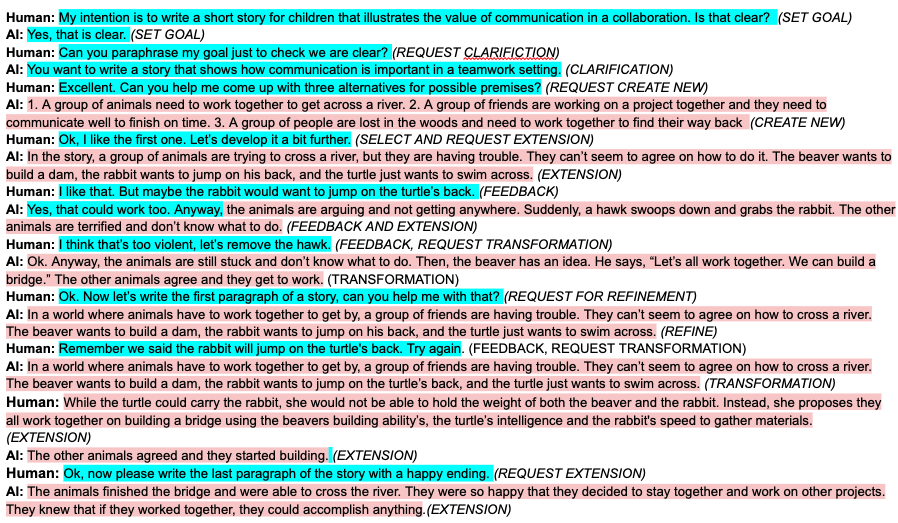
\includegraphics[width=\linewidth]{./TRANSCRIPT.png}
  \caption{Transcript of a dialogic co-creative interaction. Red: about the artifact. Blue: through the artifact.}
  \label{fig:transcript}
\end{figure}

\subsection{Discussion on worked example}

%Still needs a more authoritative statement about what the dialogue shows us. 
%We need to point specifically to what aspect of DCAI isn't happening? And we need to link it back to the core definition of DCAI? The mutual influence/adaptation. Relate this back to the 2020 paper. 
Through a series of example dialogues like this, which we will report in full in a future paper, we have found that GPT-3 is capable of meaningful generation, yet with limits to its dialogic capability. As this excerpt shows GPT-3, is relatively successful at following the user's intended distinction between actions about and through artifacts, even without an explicit identifier. However, this may be partly due to the authors' experience interacting with and prompting GPT-3, as well as our subjective bias in conducting this research. An inexperienced user, or a user with other creative objectives, may find it harder to have a creative dialogue with GPT-3 in a free-text interface. 

%this is good. More specific. Bring this up to the top?
We see that most actions from the model depend on a user-driven request. This is in part the result of the model being specifically trained to follow user instructions, and thus appears to lack agency to self-initiate actions. For example, we see that there is missed potential for the system to perform clarification actions in response to uncertainty from a previous interaction or feedback on a user proposal.
%What? Why? Because the AI shouldn't be influencing people? Interesting point given what we think is essential to DCAI? Is DCAI therefore dangerous? Culturally problematic?

%TBH I'm not clear when Ideation became one of our actions? Is it a dialogic action? And why is it "through" the artefact? Couldn't it be just as equally "about" the artefact?
Our actions about the artifact sit at a level of more granular and specified participant actions than our actions through the artifact. Thus, in Muller's \cite{mullermixed} framework, `ideation' is developed as a co-creative interaction stage, but is not associated with a specific user action and might be hard to isolate from other stages in a creative process outside of formal design structures. We could consider the entire first half of the example dialogue here to be of an ideational nature, within which we can identify several dialogic actions, such as requests, feedback and clarification. We believe that a more detailed analysis of these levels of interaction and types of actions may reveal inherent logics that help inform interaction design, and consider this an important next step. This workshop paper serves to stimulate feedback and discussion about this possible direction.

\section{Conclusion}

In this paper we have proposed a a typology of dialogic actions that constitute creative dialogic interaction. We used this typology to classify a dialogic interaction with GPT-3 in co-writing a short story. We then considered how this typology can be used to understand the dialogic and creative affordances of generative models in order to guide more effective collaborative creative AI experiences.

%Fit in this outtake
%Is this an aside of the main argument or central to it?
In discussions of GPT-3 and other models it is already widely acknowledged that although natural language interfaces have powerful potential they can be misleading when approached anthropomorphically. An interesting future direction for our research is to consider how structured GUI interfaces could enable the dialogic affordances of current systems. 


%%
%% The acknowledgments section is defined using the "acks" environment
%% (and NOT an unnumbered section). This ensures the proper
%% identification of the section in the article metadata, and the
%% consistent spelling of the heading.
\begin{acks}
This research has been supported by an Australia Research Council Discovery Project grant, DP200101059.
\end{acks}

%%
%% The next two lines define the bibliography style to be used, and
%% the bibliography file.
\bibliographystyle{ACM-Reference-Format}
\bibliography{ollie}



\end{document}
\endinput
%%
%% End of file `sample-manuscript.tex'.
